\documentclass{article}
\usepackage{amsmath, amssymb}
\usepackage[english]{babel}
\usepackage{fullpage}
\usepackage{graphicx}
\usepackage[hidelinks]{hyperref}
\usepackage[round,authoryear]{natbib}
\bibliographystyle{plainnat}
\usepackage{microtype}

\author{Dieuwke Hupkes}
\title{Experiments}
\date{}

\begin{document}

\maketitle

% \section{Intro}

\section{Datasets}

I define the following set of languages:

\begin{table}[!ht]
\begin{tabular}{lcl}
    \textbf{Name} & \textit{Numeric leaves} &  \textit{Example}\\
    \hline
    $L_2$ & 2  & ($x_1$ \textit{op} $x_1$)\\
    $L_3$ & 3  & (($x_1$ \textit{op} $x_2$) \textit{op} $x_3$)\\
    $L_4$ & 4  & (($x_1$ \textit{op} $x_2$) \textit{op} ($x_3$ \textit{op} $x_4$))\\
    \dots & &\\
\end{tabular}
\end{table}

\noindent Where $x_i\in\{-19,19\}$, and \textit{op} $\in\{+,-\}$. The meaning $y$ of e sentences is the result of the arithmetic expression expressed by the languag. We restrict the languages to include only expressions such that $y\in\{-60,60\}$.\\

\noindent We define the following subsets of the languages defined above:

\begin{table}[ht!]
\begin{tabular}{llll}
    \textbf{Name} & \textit{Restriction} & \textit{Example} \\
    \hline
    $L_i+$ & \textit{op} $==+$ & $(.(.(x_1 + x_2) + \dots x_i)$ & Structurally non ambiguous\\
    $L_i-$ & \textit{op} $==-$ & $(.(.(x_1 - x_2) - \dots x_i)$ &\\
    $L_i$right & only right branching trees & $(.(.(x_1$ \textit{op} $x_2)$ \textit{op} $x_3)$ \textit{op} $\ldots x_i)$ & Structurally non ambiguous\\
    $L_i$left & only left branching trees & $(x_1$ \textit{op} $(x_2$ \textit{op} ($\ldots$ \textit{op} $(x_{i-1}$ \textit{op} $x_i).).)$ & Structurally non ambiguous\\
\end{tabular}
\end{table}

The datasets that the networks will be trained and tested on are (subsets of) unions of the languages described above.

\section{Architectures}

I use four different architectures (explanation?):

\begin{figure}[!ht]
\setlength{\tabcolsep}{18pt}
\begin{tabular}{|cccc|}
    \hline
    \textbf{A1} & \textbf{A2} & \textbf{A3} & \textbf{A4}\\
    & & &\\
    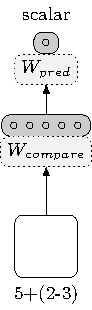
\includegraphics[scale=0.9]{A1} &
    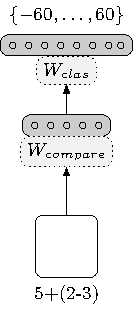
\includegraphics[scale=0.9]{A2} &
    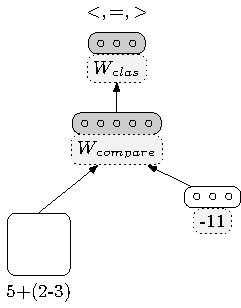
\includegraphics[scale=0.9]{A3} &
    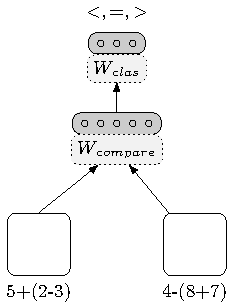
\includegraphics[scale=0.9]{A4}\\
\hline
\end{tabular}
\end{figure}


\section{Experiments}

I will start by running a sequence of experiments to determine if the networks can learn to compose the meaning of sentences from the structurally non ambiguous languages $L_2$, $L_3+$, $L_3left$ and $L_3right$. Depending on the results I will move on to more complicated languages
In principle, I would like to do all (possible) combinations that can be made by combining elements from the following table,\footnote{Of course excluding non-sensical combinations, such as Gray encoding in two dimennions} starting with architectures A1 and A2 and then expanding to A3 and A4.

\begin{table}[!ht]
\begin{tabular}{|c|c|c|c|c|c|}
    \hline
    \textbf{Network} & \textbf{Language} & \textbf{Architecture} & \textbf{Dimensionality} & \textbf{Initialisation} & \textbf{Embeddings}\\
    \hline
    SRN & $L_2$   & A1    & 10    & Random    & fixed\\
    GRU & $L_3+$  & A2    & 6     & Gray      & trained\\
    LSTM & & A3    & 2     & one-hot? &\\
    & $L_3right$ & A4    & & &\\
    & $L_3left$ &    & & &\\
    \hline
\end{tabular}
\end{table}

\section{Results}

General settings I am using for all simulations: hidden size = 20, size comparison layer = 10, batch size = 24, optimizer = adagrad.

\subsection{L2}

I ran a few run with Architecture 1, size\_hidden = 20, size\_compare=10, size\_embeddings = 2 and language = L2. 
The trainingset contains 1800 sentences, validation set contains 200 sentences, batchsize during training was 24. 
During most runs the prediction error (= the sum squared differences between the true outcome and the rounded scalar prediction of the network) on the validation set stays high for a while and then rapidly decreases to a value close to 0. 
Examples of learned embeddings are depicted in \ref{fig:L3_embeddings} and \ref{fig:L3_embeddings2}.

\begin{figure}[!ht]
        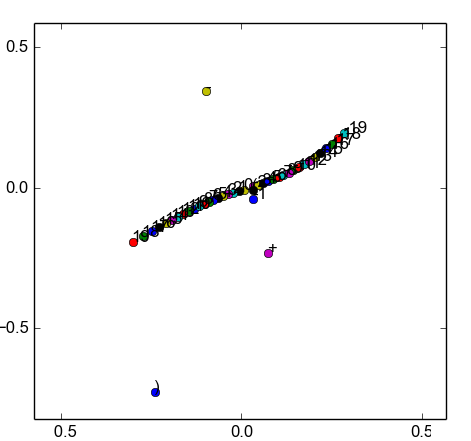
\includegraphics[scale=0.9]{L2_embeddings.png}
        \caption{Learned embeddings for network trained on 1800 L2 sentences and tested on 200 different L2 sentences. After training, the mean squared prediction error on the 200 sentences in the validation set was 0.05}\label{fig:L3_embeddings}
\end{figure}

\begin{figure}[!ht]
        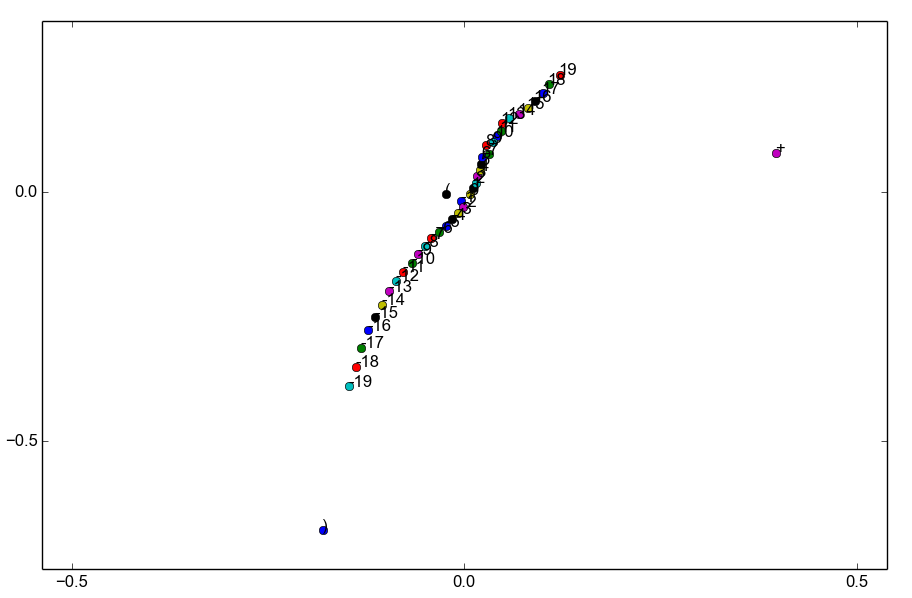
\includegraphics[scale=0.5]{L2_embeddings2.png}
        \caption{Learned embeddings for network trained on 1800 L2 sentences and tested on 200 different L2 sentences. After 1500 epochs, the mean squared prediction error on the 200 sentences in the validation set was 0.76}\label{fig:L3_embeddings2}
\end{figure}

\subsection{Training L+ languages SRN}

I did a couple runs with structurally unambiguous plus languages. 
Settings of the network were still the same: size\_hidden = 20, size\_compare=10, size\_embeddings = 2. 
I trained for 1000 epochs.\\

The numbers are still more or less ordered, but not as strongely as before. 
The brackets and + do not get a meaningful embedding (they are both very close to 0), which is sensible because in the + languages they do not contribute to the meaning of the sentence.
Examples of learned embeddings are shown in Figure \ref{fig:SRN_L2L3L6_testL5} and Figure \ref{fig:SRN_L2L3L4_testL5}.\\

It seems the simple recurrent network does not really learn a very general solution for the addition operator: when the sentence length of the test items is shorter than the longest training item (even though the exact length was not in the trainingset) the network performs the task with a very low training error. 
When the sentence length is longer than the longest training item, the network does not learn to perform the task.

\begin{figure}[!ht]
        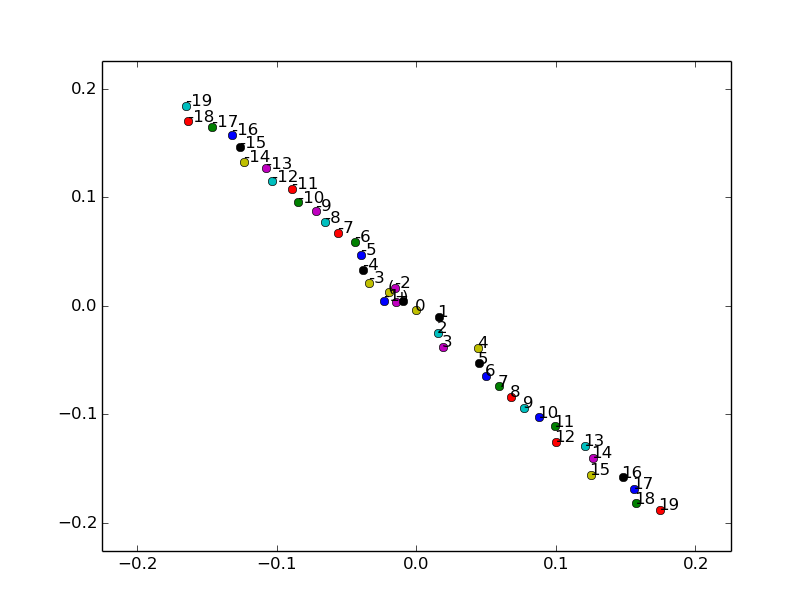
\includegraphics[scale=0.8]{SRN_L2L3L6.png}
        \caption{Learned embeddings for SRN trained on 2000 L2+ sentences, 2000 L3+ sentences and 2000 L6+ sentences, and tested on 500 L4 sentences. After 1000 epochs, the mean squared prediction error on the 200 sentences in the validation set was 0.056}\label{fig:SRN_L2L3L6_testL5}
\end{figure}

\begin{figure}[!ht]
        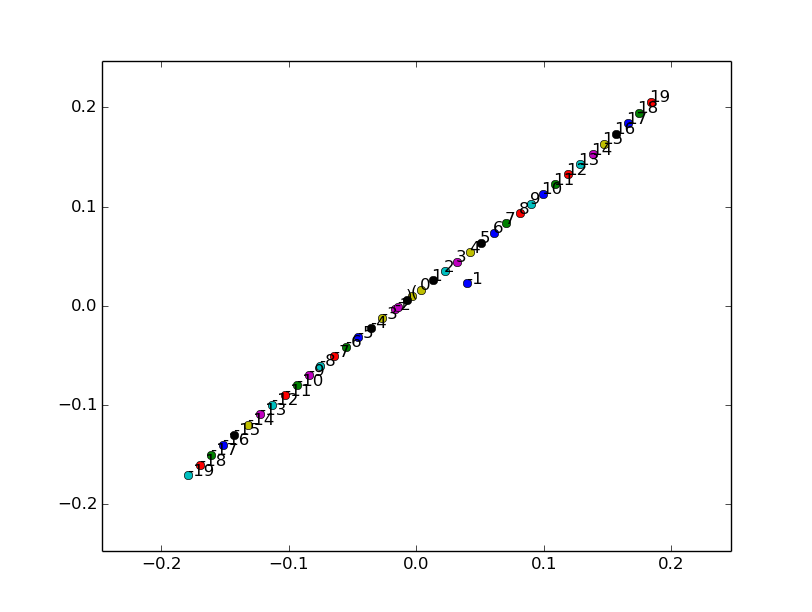
\includegraphics[scale=0.8]{SRN_L2L3L4.png}
        \caption{Learned embeddings for SRN trained on 2000 L2+ sentences, 2000 L3+ sentences and 2000 L4+ sentences, and tested on 500 L5+ sentences. After 1000 epochs, the mean squared prediction error on the 200 sentences in the validation set was 24.1 (the mspe of the trainingset was 0.006).}\label{fig:SRN_L2L3L4_testL5}
\end{figure}

\begin{figure}[!ht]
        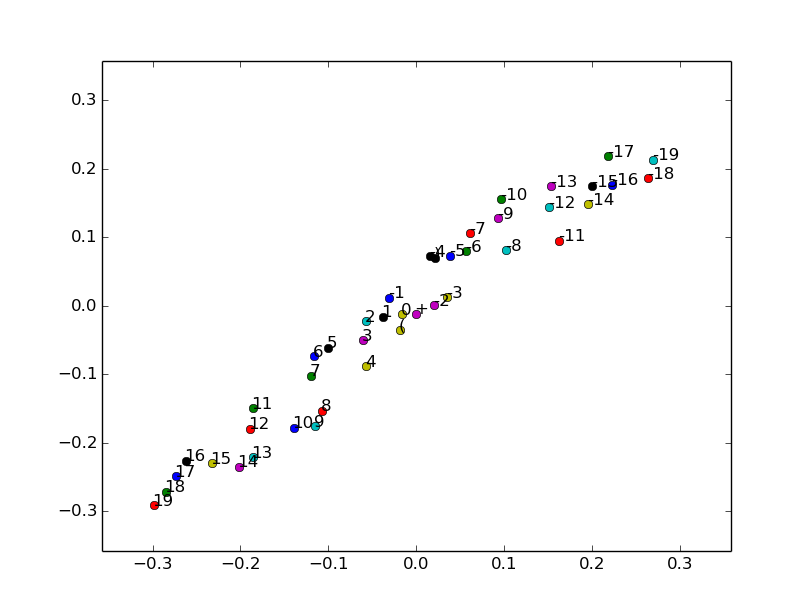
\includegraphics[scale=0.8]{GRU_L2L3L4.png}
        \caption{Learned embeddings for network with GRU layer trained on 2000 L2+ sentences, 2000 L3+ sentences and 2000 L4+ sentences, and tested on 500 L5+ sentences. After 1000 epochs, the mean squared prediction error on the 200 sentences in the validation set was 0.04}\label{fig:GRU_L2L3L4}
\end{figure}

\begin{figure}[!ht]
    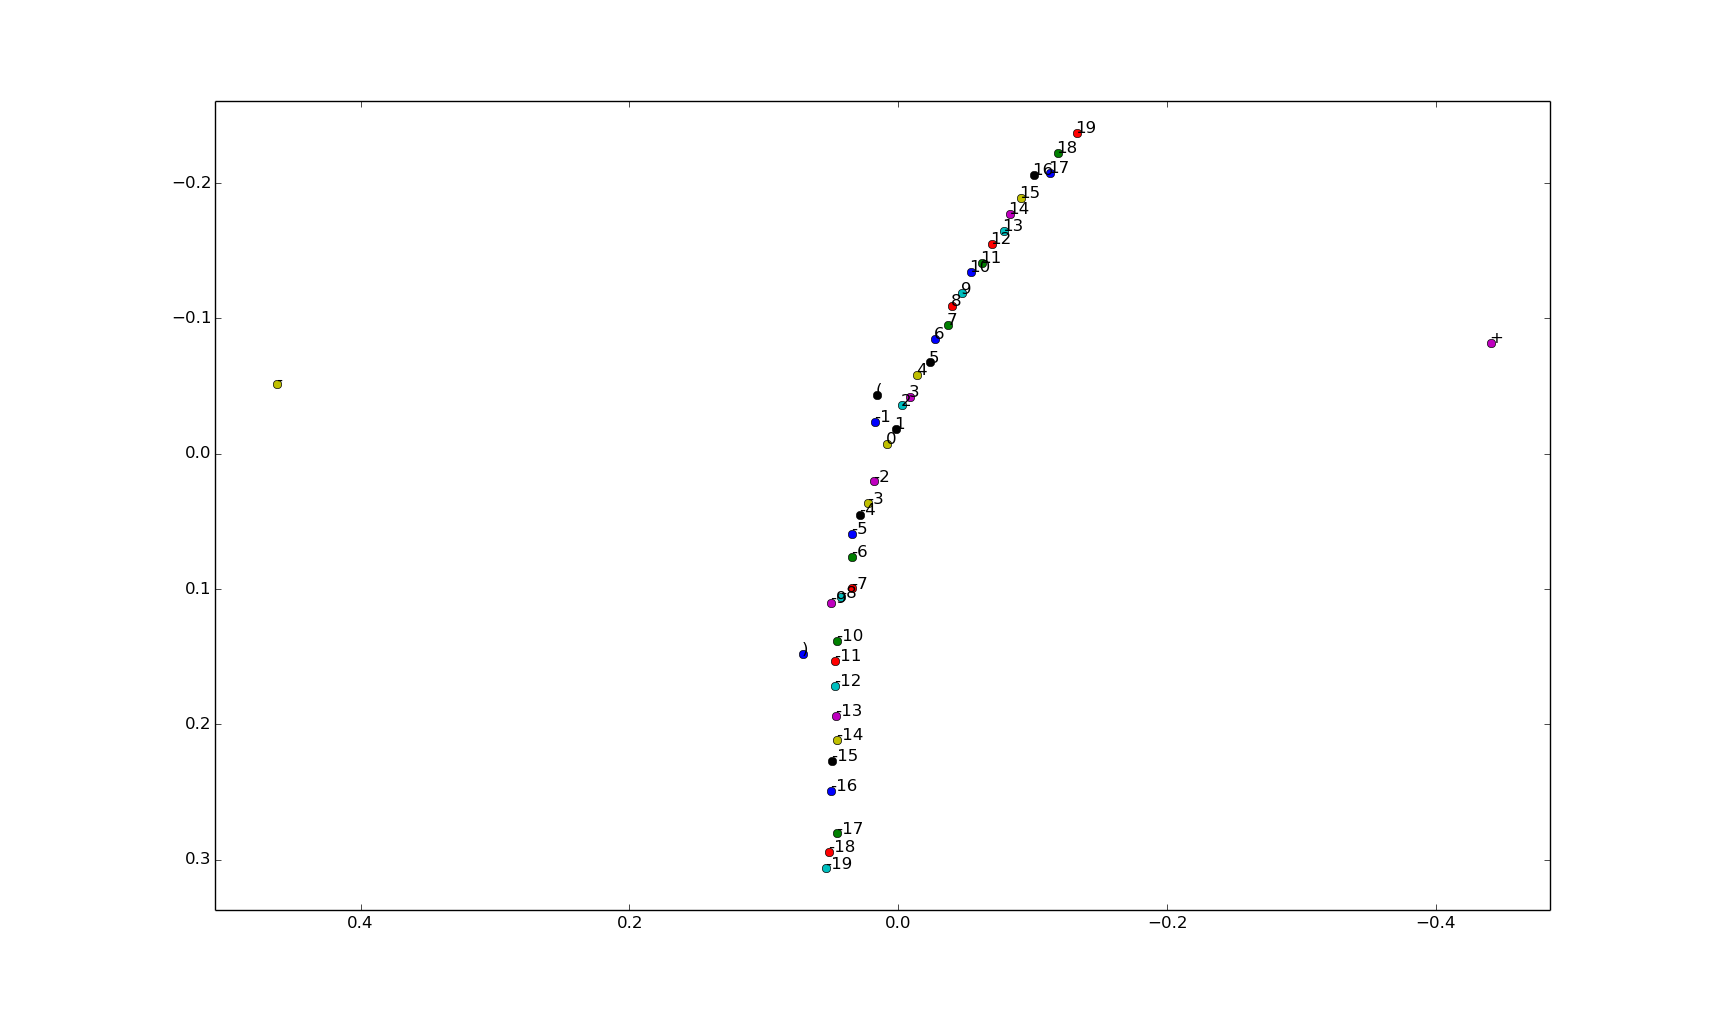
\includegraphics[scale=0.5]{SRN_L3left.png}
    \caption{Simple recurrent layer getraind op L3left, training error was nog tamelijk hoog (rond de 5).}
\end{figure}

\end{document}
